\apendice{Plan de Proyecto Software}

\section{Introducción}

La planificación y el seguimiento de metodologías de desarrollo es esencial para el éxito de cualquier proyecto. En esta sección se describirá la planificación temporal que se ha seguido del proyecto, así como el estudio de viabilidad del mismo.

\section{Planificación temporal}

Para la realización del proyecto se ha optado por la utilización del método \textbf{Scrum}, una metodología ágil de gestión de proyectos en la  que se ha dividido el desarrollo en \textbf{sprints} de aproximadamente 2 semanas de duración en la que había una reunión con el tutor y se planteaban las próximas tareas que se iban a realizar.

Para la organización de tareas se utilizó una tabla con 6 columnas:

\begin{itemize}
    \item \textbf{Procut Backlog}: En esta columna se colocan las tareas que se han de realizar a lo largo del proyecto.
    \item \textbf{Sprint Backlog}: Al inicio de cada sprint se mueven a esta columna las tareas que se planea realizar durante el transcurso de dicho sprint.
    \item \textbf{In Progress}: En esta columna se encuentran todas aquellas tareas que se están realizando en ese momento.
    \item \textbf{Review/QA}: Cuando en alguna tarea sea necesario realizar una revisión por parte del propio desarrollador cómo por parte del tutor se mueve a esta columna.
    \item \textbf{Done}: Cuando las tareas ya han sido finalizadas se mueven a esta columna
    \item \textbf{IceBox}: En esta última columna se colocan las tareas que han sido abandonadas o que tienen muy baja prioridad.
\end{itemize}


La planificación de las tareas se puede consultar en GitHub en el repositorio: \url{https://github.com/dmh1001/TFG-Monitorizacion-IOT}

Debido a la situación actual del COVID-19 las reuniones se llevaron a cabo mediante videollamadas por \textbf{Microsoft Teams}

\subsection{Sprint 0 - Introducción (30/11/2020 - 14/12/2020)}

Durante este \textbf{Sprint} lo principal fue investigar sobre las posibles herramientas que se podrían utilizar en este proyecto así cómo documentar dichas herramientas en la memoria.

Durante esta parte del proyecto se creó el repositorio de Github y se instaló ZenHub para gestionar las issues del proyecto.

\subsection{Sprint 1   (14/12/2020 - 04/01/2021 )}

Durante este \textbf{Sprint} se especificaron cuáles serían los objetivos del proyecto, se decidieron las herramientas que se iban a utilizar y se comenzó con su documentación en la memoria.

\subsection{Sprint 2   (04/01/2021 - 06/02/2021 )}

Durante este \textbf{Sprint} se instaló el servidor PRTG en una máquina virtual Windows 10 así cómo Elasticsearch. 

\subsection{Sprint 3   (06/02/2021 - 25/02/2021 )}

Durante este \textbf{Sprint} se instaló Elasticsearch, programa el cual serviría de BBDD y monitorización de nuestros sensores, en un equipo con sistema Window y se procedió a conectarlo con PRTG. 

\subsection{Sprint 4   (25/02/2021 - 12/03/2021 )}
Durante este \textbf{Sprint} se migro Elasticsearch a una máquina Virtual Ubuntu server para poder simular un servidor real.


\subsection{Sprint 5   (12/03/2021 - 26/03/2021 )}

Durante este \textbf{Sprint} se fue estructurando y creando el manual de instalación con lo desarrollado hasta la fecha.

\subsection{Sprint 6 - Conectividad PRTG-ELK (28/03/2021 - 12/04/2021 )}
En este \textbf{Sprint} se finaliza con la conexión entre PRTG y Elasticsearch, Se idea una forma de transformar los datos procedentes de PRTG mediante un sencillo programa en Flex para que los datos sean más fáciles de leer por logstash.

Con los datos obtenidos y almacenados el Elasticsearch se pudo empezar a monitorizar los datos gracias a Kibana

\subsection{Sprint 7 - acercamiento machine learning  (12/04/2021 - 26/04/2021 )}
En este \textbf{Sprint} se investigó las diferentes librerías y técnicas  
de machine learning y predicción de datos.

\subsection{Sprint 8 (1/05/2021 - 10/05/2021 )}
En este \textbf{Sprint} se configuró los sensores de la bodega y se desarrolló una función que permitía descargar los datos de Elasticsearch al servidor.

Además, se realizaron diversas pruebas y tutórales con algoritmos de machine learning para aprender y decidir cuáles serían los más apropiados en el proyecto.

\subsection{Sprint 9   (15/05/2021 - 10/06/2021 )}

En este \textbf{Sprint} se creó el modelo y se desarrolló una función capaz de devolver los datos predichos por el modelo a Elasticsearch para poder ser visualizados.

\subsection{Sprint 10  (10/06/2021 - 24/06/2021 )}
En este \textbf{Sprint} se realizaron una seré de funciones que permitían guardar y cargar el modelo al programa.

También se refactorizó el código para aumentar su legibilidad y mantener un formato y una coherencia.

\subsection{Sprint 11  (31/08/2021 - 14/09/2021 )}
En este \textbf{Sprint} se implementaron nuevos modelos y se facilitó la creación de otros en el futuro.

Se detecto un error a la hora de descargar los datos de PRTG y transformar los datos y se decidió migrar la funcionalidad de transformación de datos de Flex a Python.

Se fue redactando la memoria para dejarla finalizada para la entrega.


\begin{figure}[h]
	\centering
	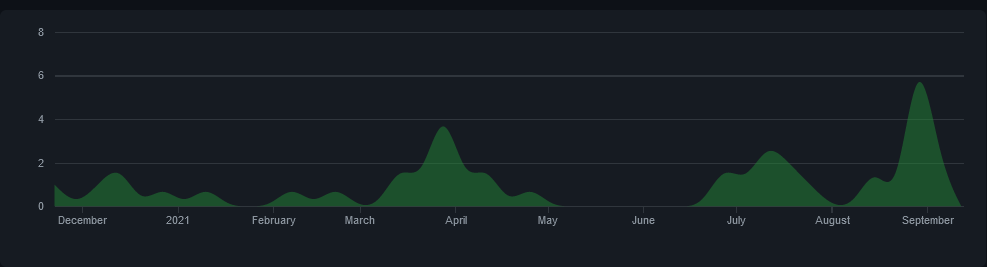
\includegraphics[width=1.1\textwidth]{img/img_grafico_github.png}
	\caption{Gráfico de commits realizados en el tiempo}
	\label{img_grafico_github}
\end{figure}
\newpage

\section{Estudio de viabilidad}

Antes de adentrarse en la realización de cualquier proyecto se ha de estudiar su viabilidad en el mercado, estimar que costes se van a tener y que beneficios se van a obtener. Durante este apartado se verá la viabilidad tanto económica como legar del proyecto.

\subsection{Viabilidad económica}
A continuación, se hará un estudio sobre los costes y beneficios del proyecto si este se hubiera realizado en un ambiente empresarial real.

\subsubsection{Costes}

\subsubsubsection{\textbf{Costes personales}}

El desarrollo del proyecto ha sido realizado por un desarrollador junior, suponiendo que el salario bruto mensual es de 2000€.

\tablaSmallSinColores{Costes de personal}{p{6.4cm} p{2.15cm} p{8cm}}{costes personales}{
  \multicolumn{1}{p{4.5cm}}{\textbf{Concepto}} & \textbf{Coste{}}\\
 }{
Salario mensual neto  & \multicolumn{1}{r}{1217.25}\\
Retención IRPF (15\%) & \multicolumn{1}{r}{216.75}\\
Seguridad social  (28.3\%) & \multicolumn{1}{r}{566}\\
Salario mensual bruto  & \multicolumn{1}{r}{2000}\\\hline
\textbf{Coste total (6 meses)}  & \multicolumn{1}{r}{12000}\\
}

\subsubsubsection{\textbf{Costes hardware}}

En este apartado se mostrará el coste de los dispositivos hardware empleados para el desarrollo del proyecto. Dado que este se ha realizado durante 8 meses y suponiendo que la amortización es de 4 años.
  
\tablaSmallSinColores{Coste hardware}{p{3.4cm} p{1.15cm} p{4cm}}{Coste hardware}{
  \multicolumn{1}{p{4.5cm}}{\textbf{Concepto}} & \textbf{Coste{}} & \textbf{Amortización{}}\\
 }{
  Ordenador  & \multicolumn{1}{r}{1200€} & \multicolumn{1}{r}{50€}\\
  }
  
\subsubsubsection{\textbf{Costes software}}

En este apartado se revisarán los costes asociados a licencias de software no gratuitos. Consideraremos que la amortización del software es de 2 años.

\tablaSmallSinColores{Coste Software}{p{3.4cm} p{1.15cm} p{4cm}}{Coste Software}{
  \multicolumn{1}{p{4.5cm}}{\textbf{Concepto}} & \textbf{Coste} & \textbf{Amortización}\\
 }
 {
  Windows 10 pro  & \multicolumn{1}{r}{259€} & \multicolumn{1}{r}{5.4€}\\
   \multicolumn{1}{r}{}\\
  }
  
\subsubsection{Beneficios}

Al tratarse de un proyecto estudiantil es muy complicado estimar un beneficio. 

\subsection{Viabilidad legal}

Para poder distribuir un producto software es necesario cumplir ciertas obligaciones legales como son el caso de las licencias.

A continuación, se mostrarán las licencias del software empleado.


\tablaSmallSinColores{Licencias}{p{4.4cm} p{6.15cm} p{4cm}}{licencias}{
  \multicolumn{1}{p{4.5cm}}{\textbf{Herramienta}} & \textbf{Licencia}\\
 }
 {
  Elasticsearch  & \multicolumn{1}{r}{}\\
  PRTG  & \multicolumn{1}{r}{}\\
  virtualBox  & \multicolumn{1}{r}{}\\
  Ubuntu  & \multicolumn{1}{r}{}\\
  Windows 10  & \multicolumn{1}{r}{}\\
  Git  & \multicolumn{1}{r}{GPL2}\\
  GitHub  & \multicolumn{1}{r}{Propietaria/Privativa}\\
   \multicolumn{1}{r}{}\\
  }
